\documentclass{article}
\usepackage{graphicx}

\usepackage{fancyhdr}
\pagestyle{fancy}
\usepackage[utf8]{inputenc}
\usepackage{lmodern}
\usepackage[a4paper]{geometry}

\begin{document}

\lhead{Relatório - Algoritmos em grafos}
\quad\\
Nome: Marcos Vinicius do Carmo Sousa\\
NUSP: 9298274\\

O exercicío foi realizado utilizando a função GRAPHrand2 (int V, int A)\\
Que recebe um numero V de vértices e A de arestas e forma um grafo aleatório
com V vértices e um número esperado A de arestas.\\
Os testes variam de acordo com o número de vértices, o numero de arestas e \\
probabilidade de que dois vértices aleatórios estão ao alcance um do outro torna-se bastante alta.

Para tal, $2<=V<=100$, onde V é o numero de vértices, $1<=A<=(V*(V-1))/2$, onde A é o numero de arestas que varia entre 1 até o máximo em um grafo não dirigido.\\
A "probabilidade alta" com que dois vertices aleatórios estao ao alcance um do outro é fornecida na linha de commando e varia de 1 a 100. \\
Assim são realizados varios testes que verificam com quantas arestas A ao menos são para vertices V necessárias para que satisfaça a probabilidade bastante alta colocada no linha de comando.\\

Foram gerados gráficos com essa relação para diferentes valores de probabilidade que dois vértices aleatórios estão ao alcance um do outro.


Observando os resultados, principalmente o de 75\% e o de 80\% , é possível notar uma relação próxima de no mínimo Arestas = Vértices * (Vertices-1)/2 \\

\begin{figure}[h]
	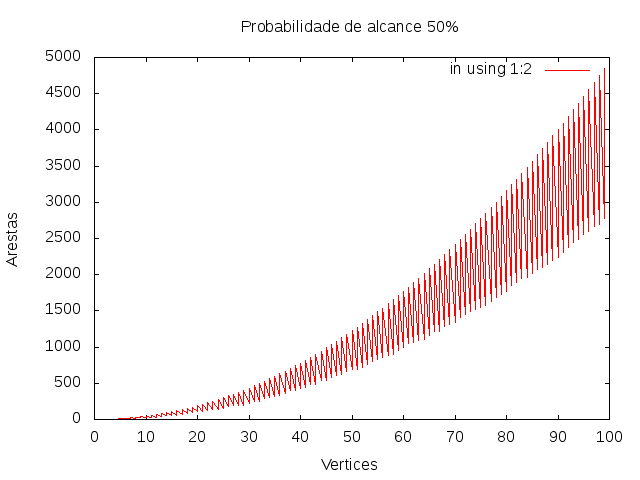
\includegraphics[width=0.9\textwidth]{50.png}
\end{figure}
\begin{figure}[h]
	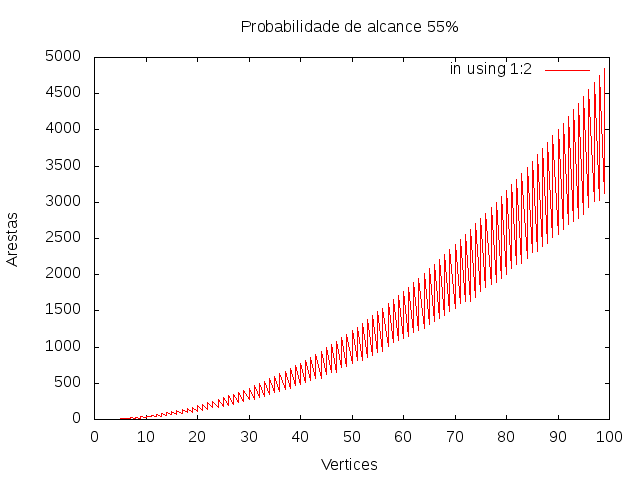
\includegraphics[width=0.9\textwidth]{55.png}
\end{figure}
\begin{figure}[h]
	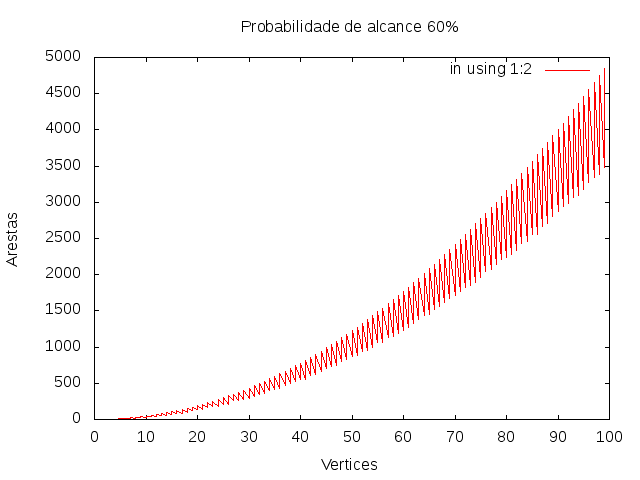
\includegraphics[width=0.9\textwidth]{60.png}
\end{figure}
\begin{figure}[h]
	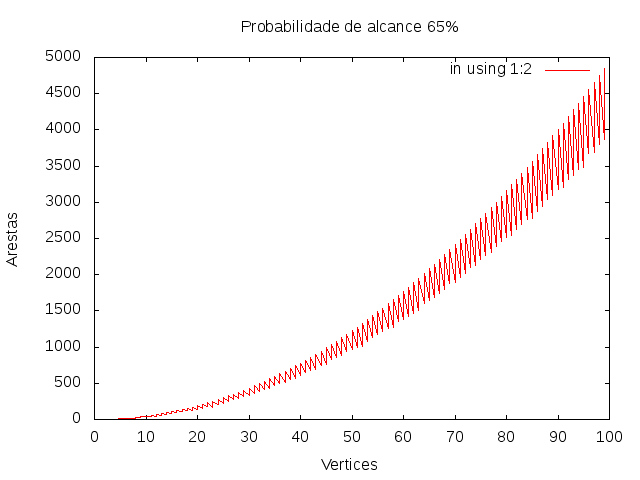
\includegraphics[width=0.9\textwidth]{65.png}
\end{figure}
\begin{figure}[h]
	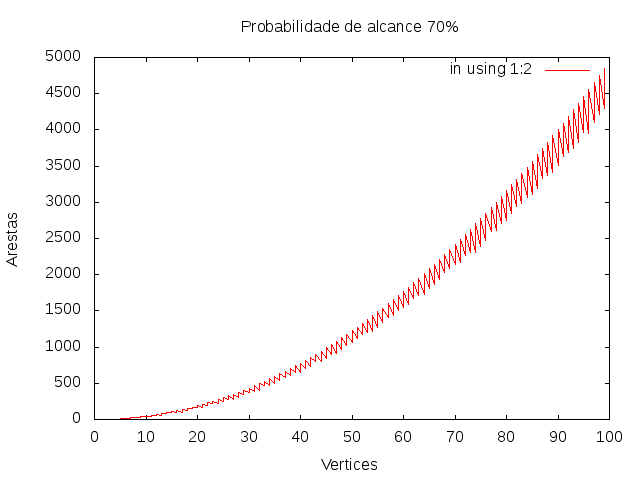
\includegraphics[width=0.9\textwidth]{70.png}
\end{figure}
\begin{figure}[h]
	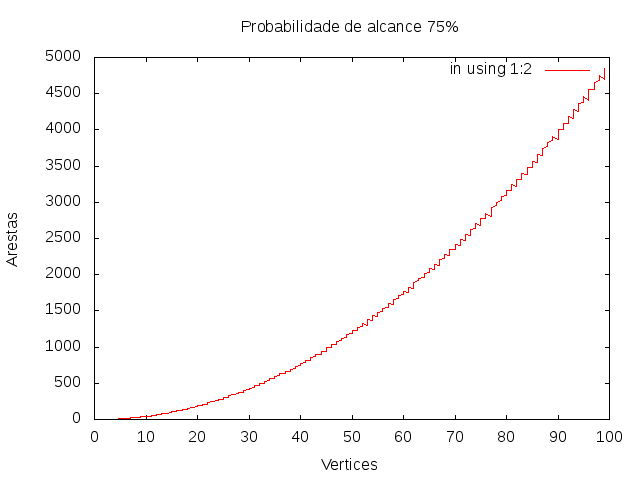
\includegraphics[width=0.9\textwidth]{75.png}
\end{figure}
\begin{figure}[h]
	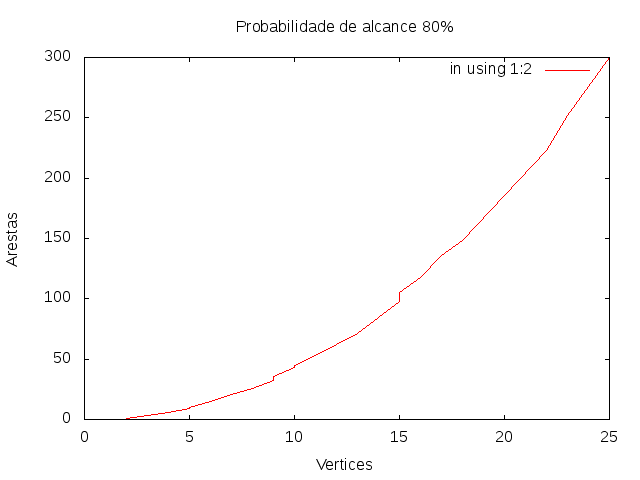
\includegraphics[width=0.9\textwidth]{80.png}
\end{figure}
\begin{figure}[h]
	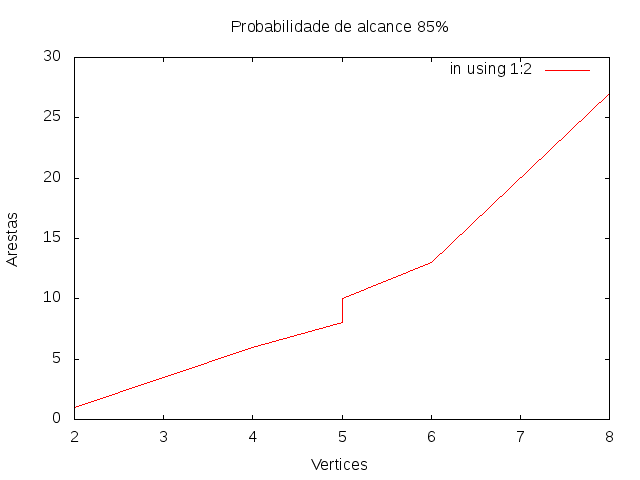
\includegraphics[width=0.9\textwidth]{85.png}
\end{figure}


\end{document}
